\chapter{Related Work}\label{Related_Work}
\thispagestyle{empty}
\setlength{\parskip}{10pt plus 5pt minus 3pt}
\setlength{\parindent}{20pt}%

In literature, we find a number of video classification strategies, each having its benefits and limitations. In this chapter we learn about the various methodologies that have been put into use for classifying videos.

\section{Gaussian Mixture Models}
Gaussian Mixture Model is a generative model for pattern recognition where it extends the basic Gaussian model to contain $k_i$ components for Class $i$. With each component is associated a different set of parameters which need to be learned separately.
\begin{enumerate}
\item Gaussian mixture models (GMMs) as used by \citet{GMM} are commonly used for classification of varying length patterns represented as sets of feature vectors. Maximum likelihood (ML) based method is commonly used for estimation of parameters of a GMM for each class, when sufficient training data is available.When the training data available for a class is limited, robust estimates of parameters can be obtained through maximum a posteriori (MAP) adaptation of a class-independent GMM (CIGMM) to the training data of each class.

\item In another methodology proposed in \citet{PCA_GMM}, the authors use statistical signal modeling approach and the PCA for the purpose of video classification using GMM. The audio and video features are taken in conjunction to form a `super' vector whose dimensionality is reduced using PCA. Then using Expectation Maximization algorithm for GMM, they model the features for the different genres.
\begin{figure}[!hbtp]
\centering
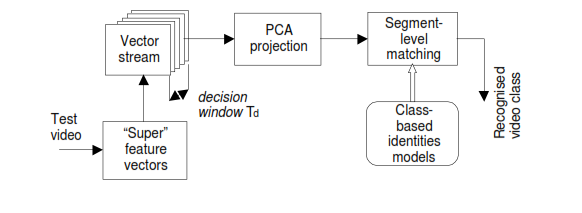
\includegraphics[scale=1]{figures/Chapter3/PCA_GMM.png}
\caption{Temporal Video Genre Classification using \cite{PCA_GMM} approach}
\end{figure}

\end{enumerate}

\section{Hidden Markov Models (HMM)}
The Hidden Markov model (HMM) is widely used for classifying sequential data. An HMM represents a set of states and the probabilities of making a transition from one state to another state.The typical usage in video classification is to train one HMM for each class. When presented with a test sequence of features, the sequence will be assigned to the class whose HMM can reproduce the sequence with the highest probability.\cite{Survey}

\begin{enumerate}
\item In \citet{CMLT}, a temporal kernel called Correlative Multilabel Temporal(CMLT) Kernel is introduced using correlative multi-label formulation which can leverage the concept interactions as well as low-level feature dynamics to boost the video event detection. It first adapts a universal reference model (URM) to a HMM for an individual video sequences.Then similarities can then be computed between these HMMs as temporal kernel based on their discrimination distances.


 
\item In the model proposed by \citet{Active} called Activity Concept Transitions in Video Events(ACTIVE), a video event is a sequence of activity concepts. A new concept is generated with certain probabilities based on the previous concept. An observation is a low level feature vector from a sub-clip and generated based on the concepts. Then the feature vector is obtained by using Fisher Kernel over the HMM. The features are then classifies using an SVM.

\end{enumerate}

\section{SVM}
SVM is one of the best and most widely used classifiers. Many classification algorithms use SVM as the main classifier after the feature selection procedure. This is primarily because SVM has a good generalization capability. We now discuss a few SVM based approaches present in literature.
\begin{enumerate}

\item \citet{Yegna} do video classification based on color, shape and motion features using support vector machine models. They use 3 types of features:-
\begin{itemize}
\item Color Features which include 3 moments of color histograms- mean, variance and skewness
\item Shape features that use edge histograms
\item Motion features where  motion is extracted by pixel-wise differencing of consecutive frames.

\end{itemize} Then using one-versus-rest approach, they use these feature vectors for SVM classification.

\item A  modified Directed Acyclic Graph Support Vector Machine (DAGSVM) model has been presented by \citet{DAGSVM} in which they have used features of editing, color,texture and motion form the video. Then, they have used one-to-one SVM that has been arranged as Directed Acyclic Graph because it yields faster performance.
\begin{figure}[!hbtp]
\centering
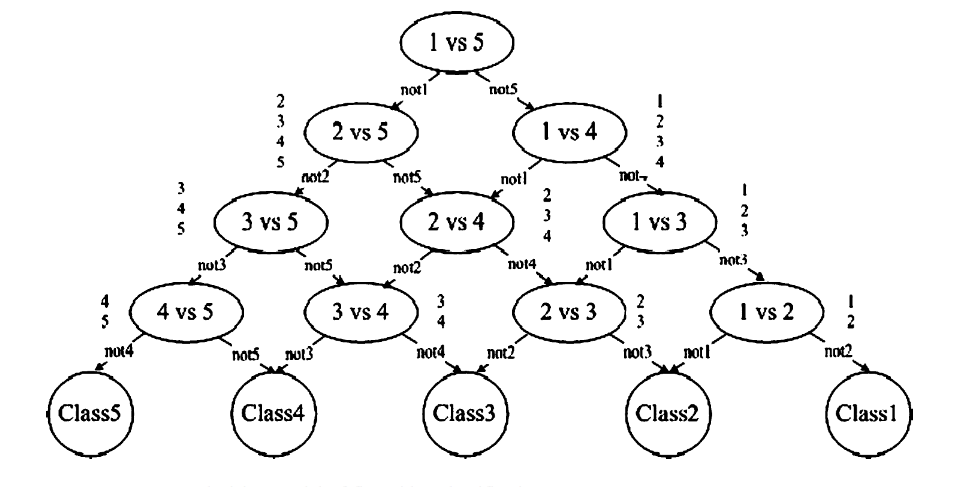
\includegraphics[scale=0.5]{figures/Chapter3/DAGSVM.png}
\caption{DAGSVM for Video Classification by \citet{DAGSVM}}
\end{figure}

\item \citet{Hierarchical_SVM} proposed an Hierarchical SVM scheme that uses ten computable spatio-temporal features to distinguish the different genres This model consists of a series of SVM classifiers united in a binary-tree form.  This scheme used 2 types of features:
\begin{itemize}
\item Temporal Features  which include average shot length, cut percentage, average color difference and camera motion. 
\item Spatial Features which include face frames ratio, average brightness and average color entropy.
\end{itemize} 
\begin{figure}[!hbtp]
\centering
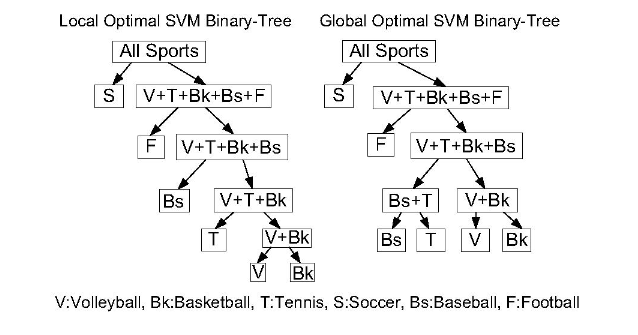
\includegraphics[scale=0.9]{figures/Chapter3/Hierarchical_SVM.png}
\caption{Local and Global optimal SVM Binary Tree by \citet{Hierarchical_SVM}}
\end{figure}
\newpage
Using these features, the proposed method creates 2 types of trees:-
\begin{itemize}
\item A local optimal SVM binary tree that attempts to find the best separation at each node using 2-fold cross-validation. which aims at finding the best separation at each node locally.
\item A global optimal SVM tree performs a global optimization of the SVM binary tree by performing the cross-validation for each possible binary tree and rhen choosing the one with the highest accuracy.
\end{itemize} 

\item In the method proposed by \citet{String_kernel}, events are modeled as a sequence composed of histograms of visual features, computed from each frame using the traditional BoW. The sequences are
treated as strings (phrases) where each histogram is considered as a character. Event
classification of these sequences of variable length, depending on the duration ofthe video clips, are performed using SVM classifiers with a string kernel that usesthe Needlemann-Wunsch edit distance. The basic idea of the algorithm is to build up the best alignment through optimal alignments of smaller subsequences, using dynamic programming,unlike other approaches, such as dynamic time warping. The proposed kernel is of the form- $ K(x,x')=\exp{(-d(x,x'))}$ where $ d(x,x') $ is the Needleman-Wunsch edit distance between $x$ and $x'$.

\begin{figure}[!hbtp]
\centering
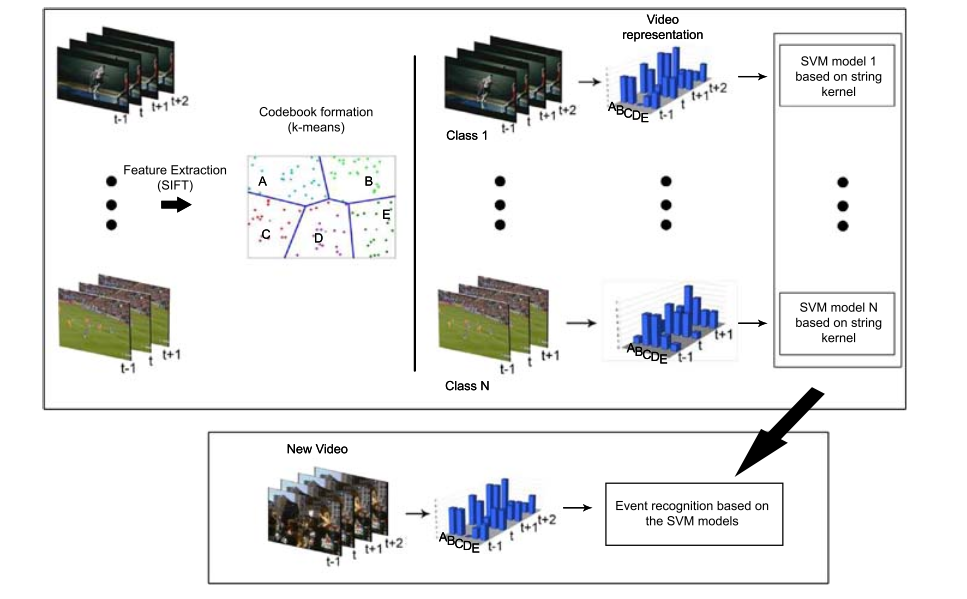
\includegraphics[scale=0.6]{figures/Chapter3/String_kernel.png}
\caption{String Kernel approach of \citet{String_kernel}}
\end{figure}


\item \citet{Motion_Words} propose the use of Motion Words for Videos for video classification.They pool features over supervoxelsby segmenting the video into supervoxels,using video segmentation . The proposed representation enables
localization of common regions across videos in both space and time that yields meaningful regions, resulting in interpretative features.

\begin{figure}[!hbtp]
 \centering
 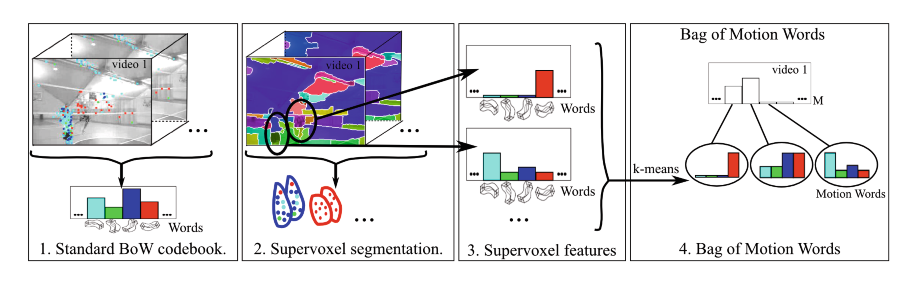
\includegraphics[scale=0.7]{figures/Chapter3/Motion_Words.png}
 \caption{Bag of Motion Words method by \citet{Motion_Words}}
 \end{figure}


For constructing the Bag of Motion Words, 
\begin{itemize}
\item Compute a standard Bag of Words code-book from low-level descriptors
\item Compute a supervoxel segmentation
\item Pool the encoded low-level descriptors in each supervoxel to obtain
supervoxel-based feature vectors
\item Cluster the supervoxel-based vectors to learn a code-book of Motion Words.
\end{itemize}  


\item \citet{Feature_Kernel} have proposed a kernel for matching feature sequences
based on the LCSS distance measure and integrating the MPEG-7 kernel. They use 4 MPEG-7 features- Color Layout (CLD), Dominant Color (DCD), Color Structure (CSD) and Edge Histogram (EHD). The joint kernel is of the form-
\begin{equation}
K_{mpeg-7}(x,x')=\Pi_{i=cld,dcd,csd,ehd} \exp{(-w_i K_i(x,x'))}
\end{equation}
where $K_i(x,x')$ is the specific kernel for each feature.Apart from kernel based on features, they have also used a kernel based on the distance of subsequences of feature vectors in order to deal with sequences of feature vectors. For this they use a kernel that is based on the \textit{longest common subsequence kernel}.


\item For the purpose of video classification,\citet{DACO} represent actions directlyas time series of frames and propose to model the event's key dynamic aspects by using auto-correlation.That is they use the cross-correlation of the signal of frames with a temporally shifted version of itself, defined as the distance measure \textit{Hilbert-Schmidt norm} of the difference between auto-correlations. The associated Gaussian RBF kernel is called the Difference between Auto-Correlation Operators (DACO) kernel. The motivation behind the DACO kernel is that the distance will tend to be smaller for time series with almost no temporal structure (e.g. for random sequences of frames) and bigger for actions with quasi-deterministic relationships between neighboring frames (e.g. a constant translation movement). 



\item Multiple kernel learning (MKL) has been proposed by \citet{MKL} for problems, where instead of choosing a kernel a priori, weights for combining different kernels are learned together with the model. Multiple kernel learning (MKL) is an approach that considers
a set of kernels potentially appropriate for their problems, and estimates both the parameters of the individual kernels as well as their relative weights during the training
phase. The weights are assigned using the interleaved optimization method.

\item \citet{Online_Concept} proposed sliding window variants of three approaches for sequence-based kernels -temporal pyramid matching, all subsequences, longest common subsequence and show how they can be efficiently applied to online concept detection by use of sliding window segmentation.
 \end{enumerate}

%\bibliographystyle{ieeetr} 
%\bibliography{biblio}
%\end{document}